%%%%%%%%%%%%%%%%%%%%%%%%%%%%%%%%%%%%%%%%%%%%%%%%
% Boissier Florian
% Fichier personel principal: boissier/rapport.tex
% L3 Info
%%%%%%%%%%%%%%%%%%%%%%%%%%%%%%%%%%%%%%%%%%%%%%%%

\chapter{Quaternions et rotation dans l'espace}
Les quaternions unitaires fournissent une notation mathématique commode pour représenter l'orientation et la rotation d'objets en trois dimensions. Comparés aux angles d'Euler, ils sont plus simple à composer et évitent le problème du blocage de cardan. Comparés aux matrices de rotations, ils sont plus stables numériquement et peuvent se révéler plus efficaces. Les quaternions ont été adoptés dans des applications en infographie, robotique, navigation, dynamique moléculaire et la mécanique spatiale des satellites.

\section{Opérations de rotation à l'aide de quaternions}
Une explication très stricte des propriétés utilisées dans cette section est donnée par Altmann\label{Altmann}.

	\subsection{L'hypersphère des rotations}
		\subsubsection{Se faire une idée de l'espace des rotations}
			Les quaternions unitaires représentent l'\emph{espace mathématique} des rotations en trois dimensions de façon relativement simple. On peut comprendre la correspondance entre les rotations et les quaternions en commençant d'abord par se faire une idée intuitive de l'espace des rotations lui-même.
Deux rotations d'angles différents et d'axes différents dans l'espace des rotations. La norme du vecteur est liée à l'amplitude de la rotation.

Chaque rotation en trois dimensions consiste à tourner d'un certain angle autour d'un certain axe. Quand l'angle est nul, l'axe n'a pas d'importance, de telle façon qu'une rotation de zéro degré est un simple point dans l'espace des rotations (c'est la rotation identité). Pour un angle petit mais non nul, l'ensemble des rotations possibles est une petite sphère entourant la rotation identité, où chaque point de la sphère représente un axe pointant dans une direction particulière (comparez avec la sphère céleste). Des rotations d'angles de plus en plus grands s'éloignent progressivement de la rotation identité, et nous pouvons nous les représenter comme des sphères concentriques de rayons croissants. Par conséquent, au voisinage de la rotation identité, l'espace abstrait des rotations ressemble à l'espace ordinaire en trois dimensions (qui peut également être vu comme un point central entouré de sphères de différents rayons. La ressemblance s'arrête là : lorsque l'angle de rotation dépasse \ang{180}, les rotations suivant les différents axes cessent de diverger et commencent à nouveau à se ressembler, pour finir par devenir identiques (et égales à la rotation identité) lorsque l'angle atteint \ang{360}.

\begin{figure}[ht]
	\centering
	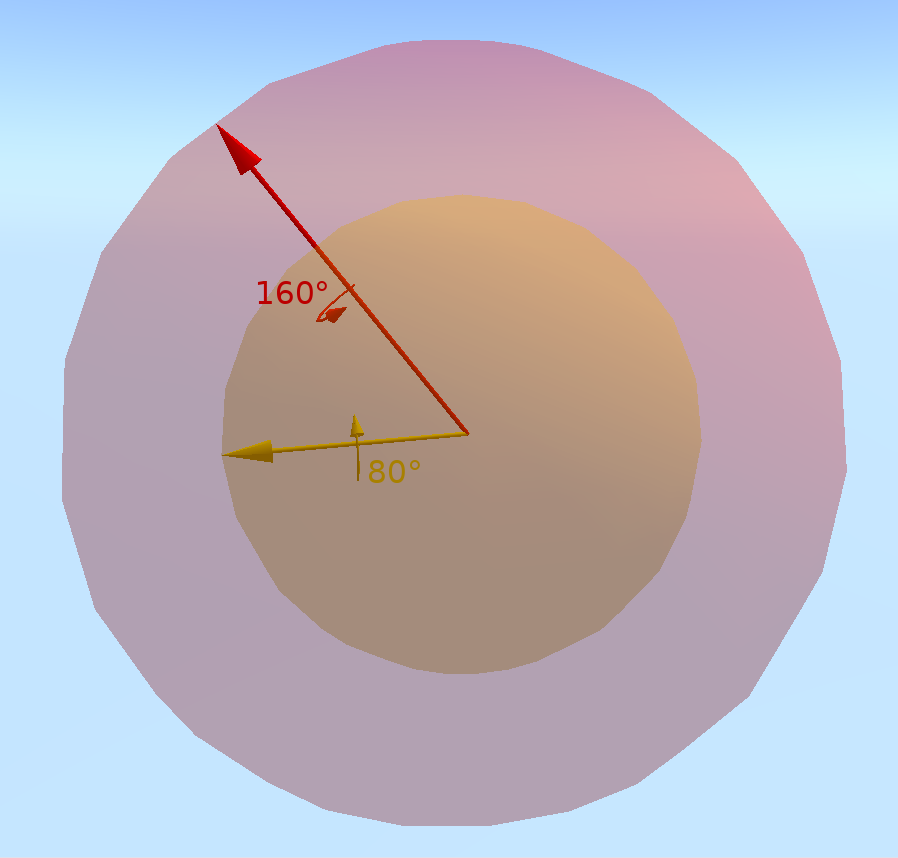
\includegraphics[width=5cm]{ressources/espace_rotations}\hfill
	\caption{Deux rotations d'angles différents et d'axes différents dans l'espace des rotations. La norme du vecteur est liée à l'amplitude de la rotation.}
	\label{espace_rotations}
\end{figure}

L'hypersphère des rotations pour les rotations d'axes horizontaux (axes compris dans le plan xy).
On constate un phénomène analogue à la surface d'une sphère. Si nous nous plaçons au pôle Nord et traçons à partir de là des lignes droites (en fait, des méridiens) dans plusieurs directions, elles divergeront puis convergeront à nouveau au pôle Sud. Des cercles concentriques de rayon croissant dessinés autour du pôle Nord (des parallèles) finiront par s'effondrer en un point au pôle Sud une fois que l'on a parcouru la distance entre les pôles. On peut assimiler les différentes directions à partir du pôle (c'est-à-dire les différents méridiens) aux différents axes de rotations et les différentes distances au pôle Nord aux différents angles : on a ainsi une analogie de l'espace des rotations. Mais la surface de la sphère est en deux dimensions alors que les \emph{axes} de rotation utilisent déjà trois dimensions. L'espace des rotations est donc modélisé par une sphère de dimension 3 dans un espace à 4 dimensions (une hypersphère). Nous pouvons penser à la sphère ordinaire comme à une section de l'hypersphère, de la même façon qu'un cercle est une section de sphère. On peut prendre la section pour représenter, par exemple, uniquement les rotations d'axes dans le plan $xy$ (voir illustration ci-contre). On remarque que l'angle de la rotation est deux fois la différence de latitude avec le pôle Nord : en effet, les points de l'équateur représentent des rotations de \ang{180}, pas de \ang{90}, et le pôle Sud représente la rotation identité de \ang{360}, et pas le demi-tour de \ang{180}.

Le pôle Nord et le pôle Sud représentent la même rotation, et en fait cela s'applique à n'importe quelle paire de points aux antipodes l'un de l'autre : si un point correspond à une rotation d'angle $\alpha$ autour de l'axe dirigé par le vecteur $\vv{v}$, l'autre point correspond à une rotation d'angle $\text{\ang{360}} - \alpha$ autour de l'axe dirigé par le vecteur $\vv{v}$. En fait, l'espace des rotations n'est pas l'hypersphère elle-même, mais l'hypersphère où l'on identifie les points aux antipodes l'un de l'autre. Mais dans un but de simplification, nous pouvons penser aux rotations comme à des points de la sphère en dimension 4, même si la moitié de ces points est redondante (revêtement double).

\begin{figure}[ht]
	\centering
	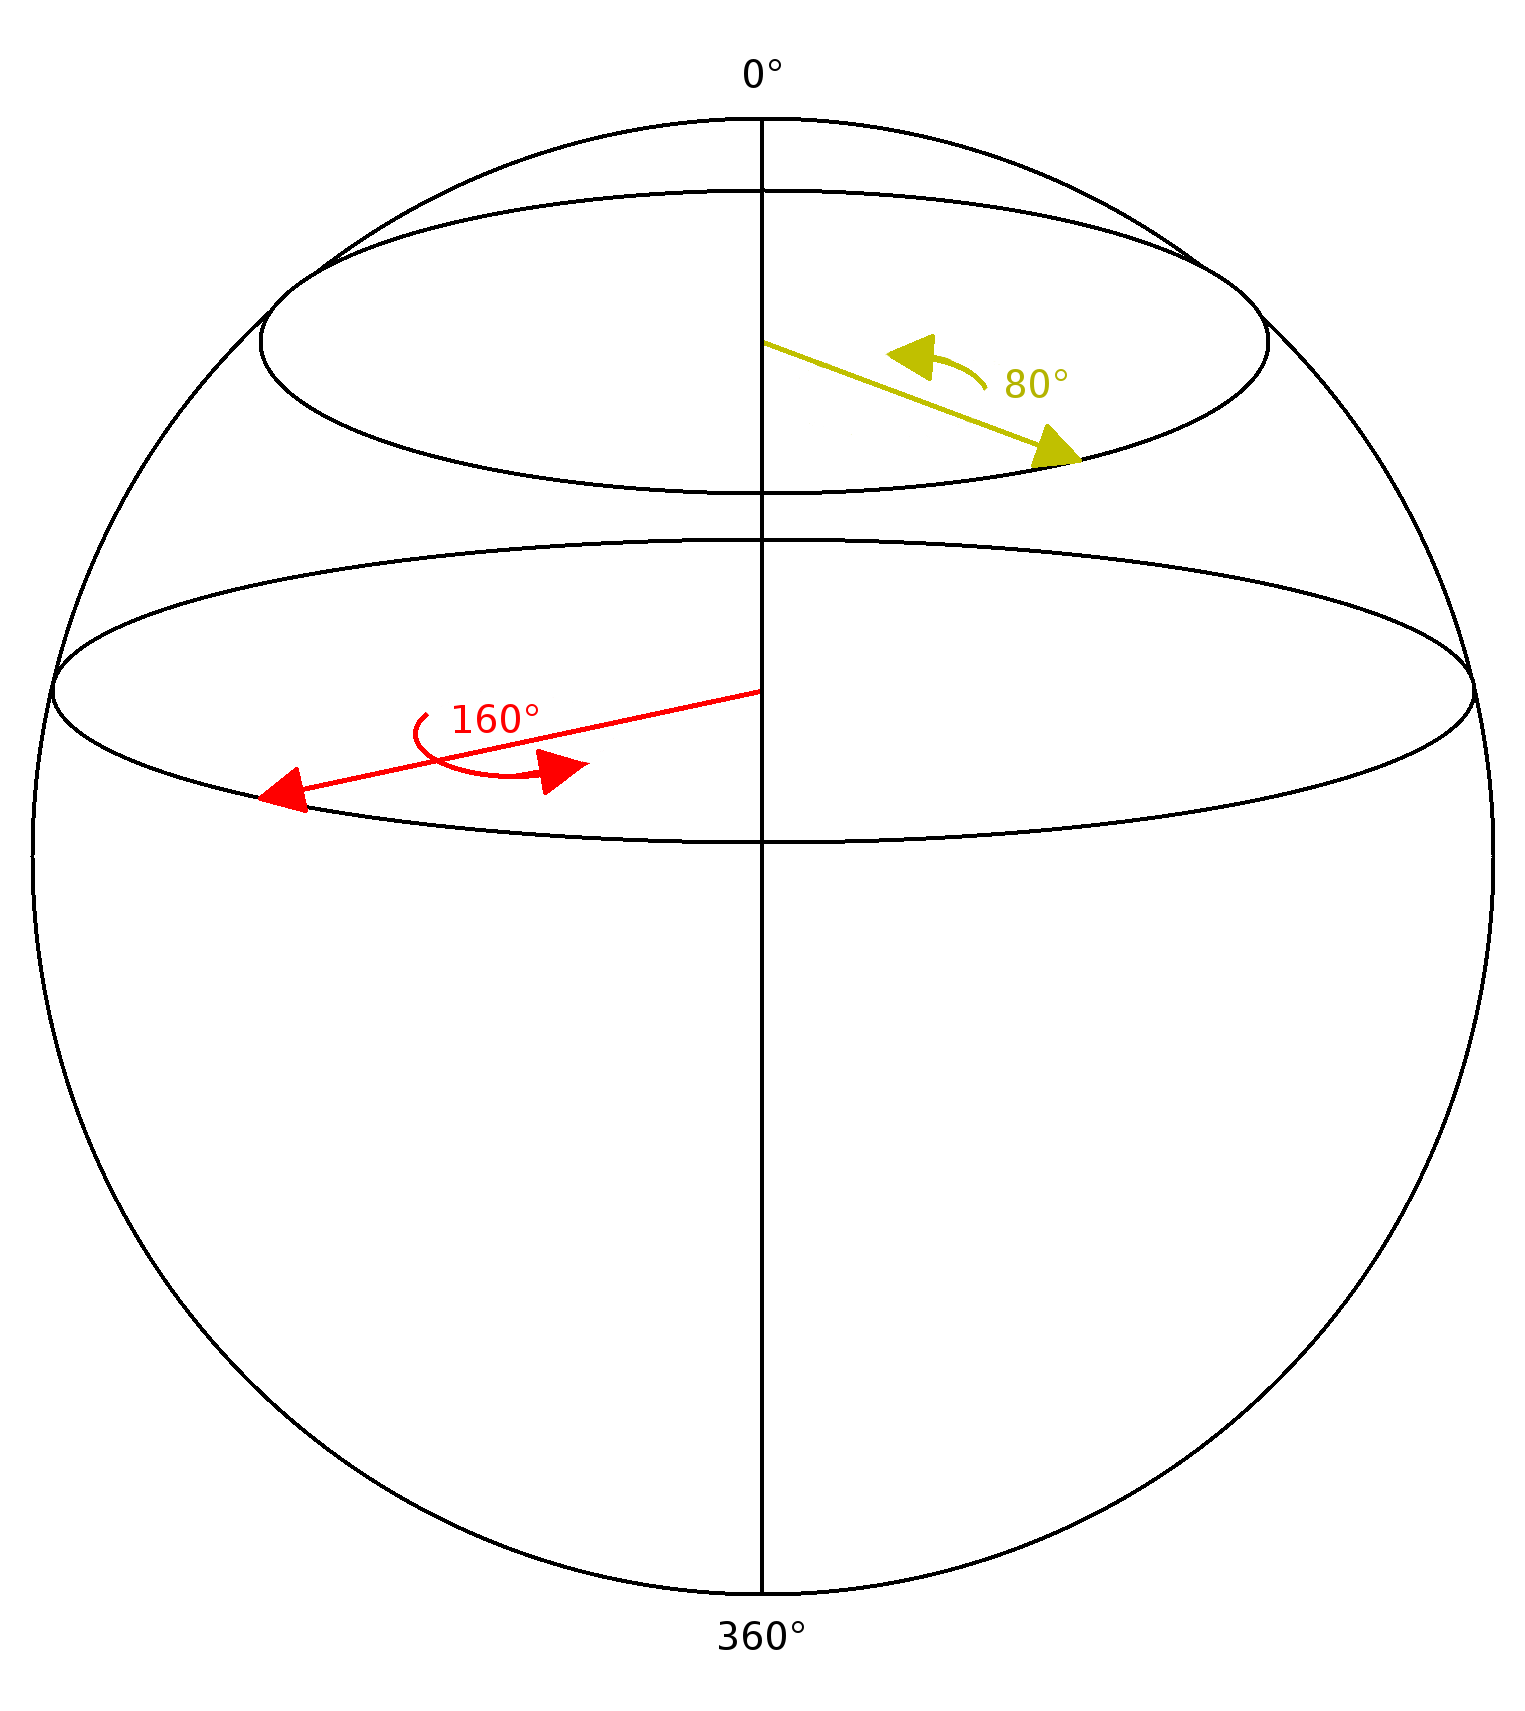
\includegraphics[width=5cm,height=4cm]{ressources/hypersphere_rotations}\hfill
	\caption{L'hypersphère des rotations pour les rotations d'axes horizontaux (axes compris dans le plan $xy$).}
	\label{hypersphere_rotations}
\end{figure}
		\subsubsection{Paramétrer l'espace des rotations}
			Nous pouvons paramétrer la surface d'une sphère à l'aide de deux coordonnées, comme la latitude et la longitude. 
Mais la latitude et la longitude se comportent mal (sont dégénérés) aux pôles Nord et Sud, 
alors que les pôles ne sont pas différents par nature des autres points de la sphère. 
Aux pôles Nord et Sud (de latitudes $+$\ang{90} et $-$\ang{90}), la longitude perd son sens.

On peut montrer qu'aucun système de coordonnées à deux paramètres ne peut éviter cette dégénérescence 
(c'est le théorème de la boule chevelue). Nous pouvons éviter de tels problèmes en plongeant la sphère 
dans l'espace à trois dimensions et en la paramétrant au moyen de trois coordonnées 
cartésiennes (ici $w$, $x$ et $y$), en plaçant le pôle Nord à $(w, x, y) = (1, 0, 0)$, 
le pôle Sud à $(w, x, y) = ( -1, 0, 0)$ et l'équateur sera le cercle d'équations 
$w = 0 \text{et} x^2 + y^2 = 1$. Les points de la sphère satisfont la contrainte $w^2 + x^2 + y^2 = 1$, 
donc nous avons toujours deux degrés de liberté, bien que l'on ait trois coordonnées. 
Un point $(w, x, y)$ de la sphère représente une rotation de l'espace ordinaire autour 
de l'axe horizontal dirigé par le vecteur $\vvv{v}{x}{y}{0}$ et d'angle 
$\alpha = 2\cos^{-1} w = 2 \sin^{-1}\sqrt{x^2+y^2}$.

De la même façon, l'hypersphère décrivant l'espace des rotations dans l'espace en trois dimensions 
peut être paramétrée au moyen de trois angles (angles d'Euler), mais tout paramétrage de ce type 
dégénère en certains points de l'hypersphère, ce qui conduit au problème du blocage de cardan. 
Nous pouvons éviter cela en utilisant quatre coordonnées euclidennes $w, x, y et z$, 
avec $w^2 + x^2 + y^2 + z^2 = 1$. Le point de coordonnées $(w, x, y, z)$ représente une rotation 
autour de l'axe dirigé par le vecteur $\vvv{v}{x}{y}{z}$
et d'angle $\alpha = 2\cos^{-1} w = 2 \sin^{-1}\sqrt{x^2+y^2+z^2}$.
	\subsection{Des rotations aux quaternions}
		\subsubsection{Les quaternions en bref}
			On peut définir les nombres complexes en introduisant un symbole abstrait $i$ qui se conforme aux 
règles usuelles de l'algèbre et qui en plus obéit à la règle $i^2 = - 1$. 
Cela suffit à reproduire toutes les règles de calcul des nombres complexes, 
par exemple: 
\[
(a + bi)(c + di) = ac + adi + bic + bidi = ac + adi + bci + bdi^{2} = (ac - bd) + (bc + ad) i
\]

De la même façon, les quaternions peuvent être définis en introduisant des symboles abstraits 
$i, j \text{et} k$ qui satisfont aux règles $i^2 = j^2 = k^2 = ijk = -1$ et les règles 
algébriques usuelles \emph{sauf} la commutativité de la multiplication (un exemple familier 
de multiplication non commutative est la multiplication des matrices). L'ensemble des règles 
de calcul découle de ces définitions ; par exemple, on peut montrer que 
\begin{align*}
(a+bi+cj+dk)(e+fi+gj+hk) &= (ae-bf-cg-dh)+(af+be+ch-dg)i+ \\
(ag+ce+df-bh)j + (ah+de+bg-cf)k.
\end{align*}

La partie imaginaire $bi+cj+dk$ d'un quaternion se comporte comme un vecteur $\vvv{v}{b}{c}{d}$
 d'un espace vectoriel à trois dimensions et la partie réelle $a$ comme un scalaire de $\mathbb{R}$.

Quand les quaternions sont utilisés en géométrie, il est pratique de les définir comme un 
scalaire plus un vecteur: $a+bi+cj+dk = a + \vec{v}$

Ceux qui ont étudié les vecteurs à un niveau élémentaire pourraient trouver étrange d'additionner 
un \emph{nombre} à un vecteur, car ce sont des objets de natures très différentes, ou de 
\emph{multiplier} deux vecteurs entre eux, car cette opération n'est d'habitude pas définie.
 Néanmoins, si l'on se souvient qu'il ne s'agit là que d'une notation pour les parties réelles et 
 imaginaires d'un quaternion, cela devient plus légitime.

Nous pouvons exprimer la multiplication de quaternions (produit de Hamilton) dans le langage moderne 
du produit vectoriel et du produit scalaire de vecteurs (qui ont en fait été inspirés au début par 
les quaternions). À la place des règles $i^2=j^2=k^2=ijk=-1$, nous avons la règle de multiplication 
de deux vecteurs $\vec{v}\vec{w}=\vec{v}\wedge\vec{w}-\vec{v}\cdot\vec{w}$, où:

\begin{itemize}
	\item $\vec{v}\vec{w}$ est la multiplication de vecteurs,
	\item $\vec{v}\wedge\vec{w}$ est le produit vectoriel (un vecteur),
	\item $\vec{v}\cdot\vec{w}$ est le produit scalaire un nombre).s
\end{itemize}

La multiplication de vecteurs n'est pas commutative (à cause du produit vectoriel), alors que la 
multiplication entre scalaires et entre un scalaire et un vecteur sont commutatives. Il découle de
 manière immédiate de ces règles que $(s + \vec{v})(t + \vec{w}) = (st - \vec{v}\cdot\vec{w}) + 
 (s\vec{w}+t\vec{v}+\vec{v}\wedge\vec{w})$.

L'inverse (à gauche et à droite) d'un quaternion non nul est $(s + \vec{v})^-1 = 
\frac{s - \vec{v}}{s^2 + \abs{\vec{v}}^2}$, comme cela peut être vérifié par calcul direct.
		\subsubsection{Relation entre les rotations et les quaternions unitaires}
			Soient $(w, x, y, z)$ les coordonnées d'une rotation, comme décrit précédemment. 
Définissons le quaternion : $q = w + xi + yj+ zk = w + \vvv{v}{x}{y}{z} = 
\cos( \alpha / 2 ) + \vec{u} \sin( \alpha/2 )$
où $\vec{u}$ est un vecteur unitaire. Soit également $\vec{v}$ un vecteur
ordinaire de l'espace en 3 dimensions, considéré comme un quaternion avec
une coordonnée réelle nulle. On peut alors montrer (voir section suivante) 
que le produit de quaternions: 
\[
q\vec{v}q^-1
\]
renvoie le vecteur $\vec{v}$ tourné d'un angle $\alpha$ autour de l'axe dirigé
par $\vec{u}$.La rotation se fait dans le sens des aiguilles d'une montre 
si notre ligne de vue pointe dans la même direction que $\vec{u}$.Cette opération 
est connue comme la conjugaison par $q$.

Il s'ensuit que la multiplication de quaternions correspond à la composition de 
rotations, car si $p \text{et} q$ sont des quaternions représentant des rotations, 
alors la rotation (conjugaison) par $pq$ est:
\[
pq\vec{v}( pq )^-1 = pq\vec{v}q^-1p^-1 = p( q\vec{v}q^-1 )p^-1 \text{,}
\]
ce qui revient à tourner (conjuguer) par $q$, puis par $p$.

Le quaternion inverse d'une rotation correspond à la rotation inverse, car
$q^-1( q\vec{v}q^-1 )q = \vec{v}$.

Le carré d'un quaternion correspond à la 
rotation de deux fois le même angle autour du même axe. Plus généralement, 
$q^n$ correspond à une rotation de $n$ fois l'angle autour du même axe que $q$.
Cela peut être étendu à un réel arbitraire n, ce qui permet de calculer des rotations intermédiaires de façon fluide entre des rotations de l'espace, c'est
\emph{l'interpolation linéaire sphérique}.
		\subsubsection{Démonstration de l'équivalence entre conjugaison de quaternions et rotation de l'espace}
			Soit $\vec{u}$ un vecteur unitaire (l'axe de rotation) et soit 
$q = \cos \frac{\alpha}{2} + \vec{u} \sin \frac{\alpha}{2}$.

Notre but est de montrer que :

\[
	\vv{v'} = q\vec{v}q^-1 = ( \cos \frac{\alpha}{2} + 
	\vec{u} \sin \frac{\alpha}{2} ) \vv{v} ( \cos 
	\frac{\alpha}{2} - \vv{u} \sin \frac{\alpha}{2} )
\]

renvoie le vecteur $\vec{v}$ tourné d'un angle $\alpha$ autour de l'axe
dirigé par $\vec{u}$.

En développant, on obtient en effet :

\begin{align*}
	\vv{v'} & = \vv{v} \coscad + (\vec{u} \vec{v} - \vec{v}\vec{u}) \sinad \cosad- \vec{u}\vec{v}\vec{u}\sincad \\
	& = \vv{v}\coscad + 2 ( \vecsc{u}{v}) \sinad \cosad - (\vec{v}(\vec{u} 
	\cdot \vec{u})) \sincad \\
	& = \vec{v}( \coscad - \sincad ) + (\vecsc{u}{v}) (2 \sinad \cosad) + \vv{u}(\vecpr{u}{v}) (2
	\sincad) \\ 
	& = \vec{v} \cosa + (\vecsc{u}{v}) \sina + \vec{u}(\vecpr{u}{v})( 1 - \cosa ) \\
	& = (\vec{v} - \vec{u}(\vecpr{u}{v})) \cosa + (\vecsc{u}{v}) \sina + \vec{u}(\vecpr{u}{v}) \\
	& = \vec{v}_{\perp} \cosa + (\vecsc{u}{v}_{\perp}) \sina + \vec{v}_{\|}
\end{align*}

où $\vec{v}_{\perp} \text{ et } \vec{v}_{\|}$ sont les composantes de $\vec{v}$ 
respectivement orthogonale et colinéaire à $\vec{u}$. C'est là la formule de 
\bsc{Olinde Rodrigues} qui donne la rotation d'angle $\alpha$ autour de l'axe dirigé par $\vec{u}$.
	\subsection{Exemple}
	
\section{Expliquer les propriétés des quaternions à l'aide des rotations}
	\subsection{Non-commutativité}
	\subsection{Les quaternions sont-ils orientés ?}
	
\section{Les quaternions et les autres représentations des rotations}
	\subsection{Description qualitative des avantages des quaternions}
	\subsection{Conversion vers et depuis la représentation sous forme de matrice}
		\subsubsection{D'un quaternion en matrice orthogonale}
		\subsubsection{D'une matrice orthogonale en quaternion}
		\subsubsection{Quaternions optimaux}
	\subsection{Comparaisons de performances avec d'autres méthodes de rotation}
		\subsubsection{Résultats}
		\subsubsection{Méthodes utilisées}
\section{Les paires de quaternions unitaires comme rotations dans l'espace à 4 dimensions}